\documentclass[a4paper,12pt]{article}

\usepackage{amsmath}
\usepackage{amssymb}
\usepackage{graphicx}
\usepackage{listings}[language=Python]
\lstdefinestyle{mystyle}{
    breakatwhitespace=false,         
    breaklines=true,                 
    captionpos=b,                    
    keepspaces=true,                 
    numbers=left,                    
    numbersep=5pt,                  
    showspaces=false,                
    showstringspaces=false,
    showtabs=false,                  
    tabsize=2
}

\lstset{style=mystyle}

\title{Lab-02 Report}
\author{st122246}

\begin{document}

\maketitle

\section{Q1: Show Image}

\begin{figure*}
	\caption{Q1: Show Image}
	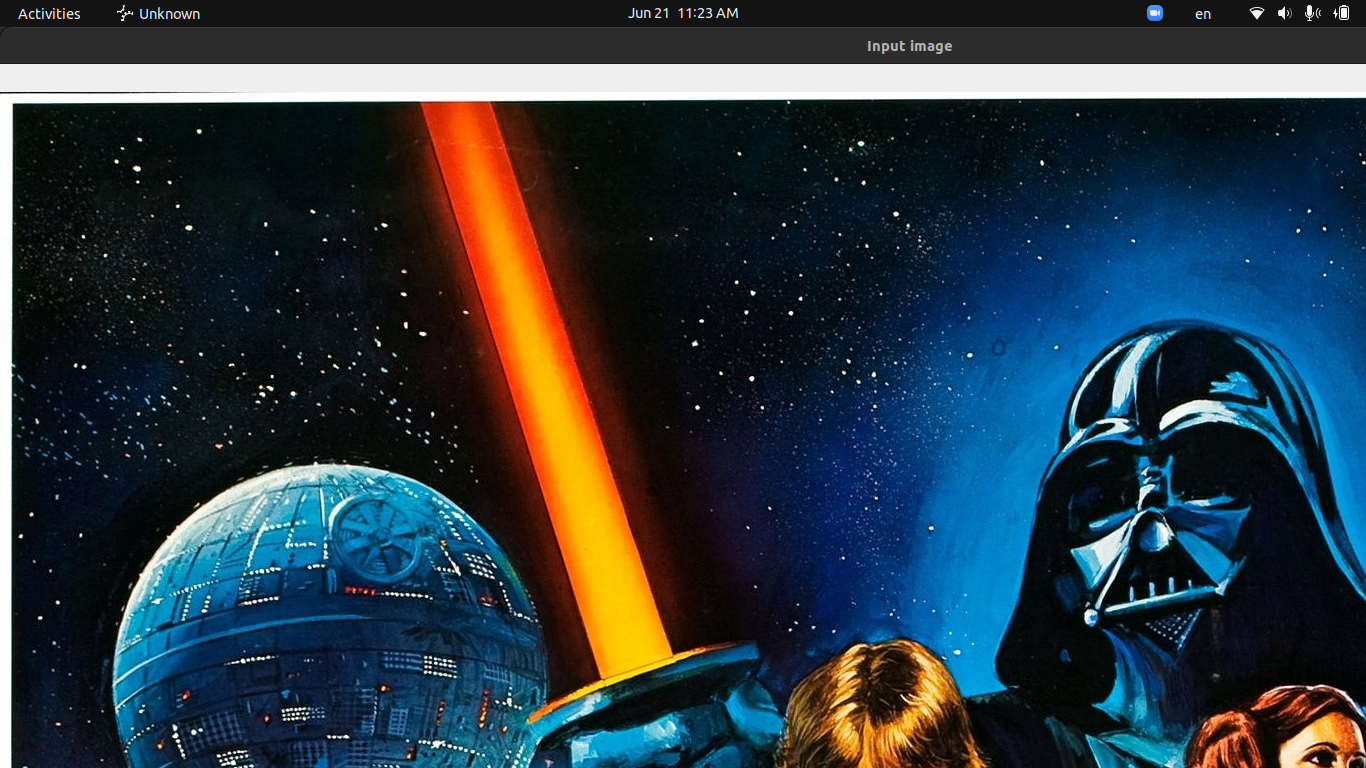
\includegraphics[scale=0.25]{img/Q1.png}
\end{figure*}

\begin{lstlisting}
import cv2 as cv

IMAGE_FILE = "../../../Data/sample.jpg"

if __name__ == "__main__":
	img = cv.imread(IMAGE_FILE)
	if img is None:
		print("Error: No image to show")

	cv.imshow("Input image", img)

	# Wait up to 5s for a key press
	cv.waitKey(5000)
	
\end{lstlisting}


\section{Q2: Show Video}
\begin{figure*}
	\caption{Q2: Show Video}
	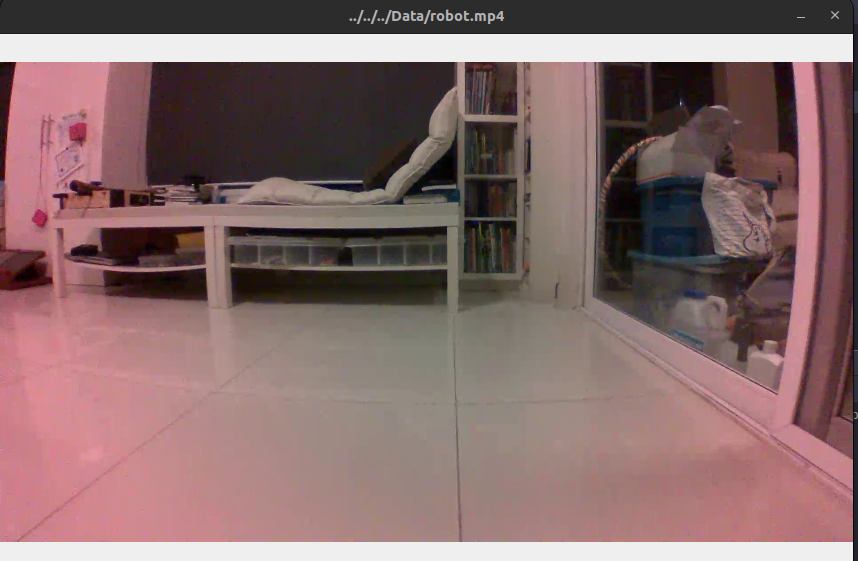
\includegraphics[scale=0.45]{img/Q2.png}
\end{figure*}
\begin{lstlisting}
import sys
import cv2 as cv

VIDEO_FILE = "../../../Data/robot.mp4"
ROTATE = False

if __name__ == "__main__":
    key = -1

    # Open video file
    videoCapture = cv.VideoCapture(VIDEO_FILE)
    height = videoCapture.get(cv.CAP_PROP_FRAME_HEIGHT)
    width = videoCapture.get(cv.CAP_PROP_FRAME_WIDTH)

    if not videoCapture.isOpened():
        print("ERROR! Unable to open \
		video file {}".format(VIDEO_FILE))
        sys.exit()

    # Capture loop
    while key != ord(' '):
        # Get the next frame
        _, matFrameCapture = videoCapture.read()
        if matFrameCapture is None:
            # End of video
            break

        # Rotate Video
        if ROTATE:
            # Rotate 180 degree and put \
			image to matFrameDisplay
            _, matFrameDisplay = cv.rotate(matFrameCapture, 
			cv.ROTATE_180)
        else:
            matFrameDisplay = matFrameCapture

        # Resize the frame
        ratio = 480.0 / height
        down_height = int(height * ratio)
        down_width = int(width * ratio)
        matFrameDisplay = cv.resize(matFrameDisplay,
                                    (down_width, down_height),
                                    ratio, ratio, cv.INTER_LINEAR)

        # Display the frame
        cv.imshow(VIDEO_FILE, matFrameDisplay)

        key = cv.waitKey(30)
\end{lstlisting}

\section{Q3: In-lab exercise 1}

\begin{enumerate}
	\item Use waitKey() to wait for the user to press <space> to advance to the next frame or 'q' to quit. Check the documentation for waitKey(), change the delay parameter to 0 for an infinite wait, and perform the necessary action on a 'spacebar' or 'q' key.
	\item Display the full 1080p or 720p frame from the video without making the display window too big for your desktop. Take a look at the documentation for namedWindow() and figure out which flags you should use to set up your display window to be resizable but keep the aspect ratio and display the expanded GUI.
	\item Next we probably want to give the user some useful information. Check out the documentation for displayOverlay() and add some explanatory information for the user about frame number, total frames, and user control actions.
	\item Last little detail: currently, if the user closes the window, the program doesn't exit.Modify your program to exit when image display window is closed.
\end{enumerate}

\begin{figure*}
	\caption{Q3: Show Video With Description}
	\includegraphics*[scale=0.275]{img/Q3.png}
\end{figure*}

\begin{lstlisting}
import sys
import cv2 as cv

VIDEO_FILE = "../../../Data/robot.mp4"
ROTATE = False

if __name__ == "__main__":
	key = ord(" ")

	# Open video file
	videoCapture = cv.VideoCapture(VIDEO_FILE)
	height = videoCapture.get(cv.CAP_PROP_FRAME_HEIGHT)
	width = videoCapture.get(cv.CAP_PROP_FRAME_WIDTH)
	totalFrameNum = int(videoCapture.get(cv.CAP_PROP_FRAME_COUNT))
	if not videoCapture.isOpened():
		print("ERROR! Unable to open video file {}".format(VIDEO_FILE))
		sys.exit()

	# Capture loop
	while True:
		# Get the next frame when press <space>
		if key == ord(" "):
			_, matFrameCapture = videoCapture.read()
			currentFrameNum = int(videoCapture.get(cv.CAP_PROP_POS_FRAMES))
			if matFrameCapture is None:
				# End of video
				break

			# Rotate Video
			if ROTATE:
				# Rotate 180 degree and put image to matFrameDisplay
				matFrameDisplay = cv.rotate(matFrameCapture, cv.ROTATE_180)
			else:
				matFrameDisplay = matFrameCapture

			# Resize the frame
			height_ratio = 768.0 / height
			width_ratio = 1366.0 / width
			down_height = int(height * height_ratio)
			down_width = int(width * width_ratio)
			matFrameDisplay = cv.resize(matFrameDisplay,
										(down_width, down_height),
										width_ratio, height_ratio,
										cv.INTER_LINEAR)

			# 1366p x 768p frame display in resizeable, keep aspect ratio, and show expended GUI
			cv.namedWindow("ROBOT.MP4", flags=cv.WINDOW_NORMAL | cv.WINDOW_KEEPRATIO | cv.WINDOW_GUI_EXPANDED)

			# Display the frame
			cv.imshow("ROBOT.MP4", matFrameDisplay)

			# Display overlay explanatory information
			explanatory_info = f"{currentFrameNum} / {totalFrameNum} " \
								f"frames. Press <space> for next frame. Press <q> to quit."
			cv.displayOverlay("ROBOT.MP4", explanatory_info)

		# Quit when press <q>
		if key == ord('q'):
			break

		# Exit program on window close
		if cv.getWindowProperty("ROBOT.MP4", cv.WND_PROP_VISIBLE) != 1:
			break

		key = cv.pollKey()
	cv.destroyAllWindows()	
\end{lstlisting}

\section{Q4: In-lab exercise 2}

\begin{figure*}
	\caption{Q4: Select 4 Points}
	\includegraphics*[scale=0.275]{img/Q4.png}
\end{figure*}

\begin{figure*}
	\caption{Q4: Estimated Homography}
	\includegraphics*[scale=0.25]{img/Q4-1.png}
\end{figure*}

\begin{figure*}
	\caption{Q4: Warped Image}
	\includegraphics*[scale=0.275]{img/Q4-2.png}
\end{figure*}

\begin{figure*}
	\caption{Q4: Warped Image and Perform Optical Flow}
	\includegraphics*[scale=0.275]{img/Q4-3.png}
\end{figure*}

\begin{lstlisting}
	import sys
	import cv2 as cv
	import numpy as np
	from os.path import exists
	
	point = (-1, -1)
	pts = []
	var = 0
	drag = 0
	mat_final = np.array([])
	mat_result = np.array([])
	
	feature_params = dict(
		maxCorners=100,
		qualityLevel=0.3,
		minDistance=7,
		blockSize=7
	)
	lk_params = dict(
		winSize=(15, 15),
		maxLevel=2,
		criteria=(cv.TERM_CRITERIA_EPS | cv.TERM_CRITERIA_COUNT, 10, 0.03)
	)
	
	color = np.random.randint(0, 255, (100, 3))
	VIDEO_FILE = "../../../Data/robot.mp4"
	ROTATE = False
	CALIBRATION_FILE = "calibration.yml"
	CALIBRATE = False
	
	
	def draw_circle_and_line(x, y):
		global point, pts, mat_result
		mat_result = mat_final.copy()
		point = (x, y)
	
		if var >= 1:
			cv.line(mat_result, pts[var - 1], point, (0, 255, 0, 255), 2)
		cv.circle(mat_result, point, 2, (0, 255, 0), -1, 8, 0)
		cv.imshow("Source", mat_result)
	
	
	def open_video(file_name):
		video_capture = cv.VideoCapture(file_name)
		if not video_capture.isOpened():
			print("ERROR! Unable to open input video file ", VIDEO_FILE)
			sys.exit('Unable to open input video file')
	
		width = video_capture.get(cv.CAP_PROP_FRAME_WIDTH)
		height = video_capture.get(cv.CAP_PROP_FRAME_HEIGHT)
		ratio = 640.0 / width
		dim = (int(width * ratio), int(height * ratio))
	
		return video_capture, width, height, ratio, dim
	
	
	def mouse_handler(event, x, y, flags, param):
		global point, pts, var, drag, mat_final, mat_result
	
		if var >= 4:
			return
	
		if event == cv.EVENT_LBUTTONDOWN:
			drag = 1
			draw_circle_and_line(x, y)
	
		if event == cv.EVENT_LBUTTONUP and drag:
			drag = 0
			pts.append(point)
			var += 1
			mat_final = mat_result.copy()
	
			if var >= 4:
				cv.line(mat_final, pts[0], pts[3], (0, 255, 0, 255), 2)
				cv.fillConvexPoly(mat_final, np.array(pts, dtype=np.int32), (0, 120, 0, 20))
			cv.imshow("Source", mat_final)
	
		if drag:
			draw_circle_and_line(x, y)
	
	
	def calibrate():
		global mat_final, mat_result, var, CALIBRATE
		CALIBRATE = True
	
		mat_pause_screen = np.array([])
		mat_frame_capture = np.array([])
		key = -1
	
		# --------------------- [STEP 1: Make video capture from file] ---------------------
		# Open video file
		video_capture, width, height, ratio, dim = open_video(VIDEO_FILE)
	
		# Capture loop
		while key < 0:
			# Get the next frame
			_, mat_frame_capture = video_capture.read()
			if mat_frame_capture is None:
				break
	
			# Rotate
			if ROTATE:
				_, mat_frame_display = cv.rotate(mat_frame_capture, cv.ROTATE_180)
			else:
				mat_frame_display = mat_frame_capture
	
			mat_frame_display = cv.resize(mat_frame_display, dim)
	
			cv.imshow("ROBOT.MP4", mat_frame_display)
			key = cv.waitKey(30)
	
			# --------------------- [STEP 2: pause the screen and show an image] ---------------------
			if key >= 0:
				mat_pause_screen = mat_frame_capture
				mat_final = mat_pause_screen.copy()
	
		# --------------------- [STEP 3: use mouse handler to select 4 points] ---------------------
		if mat_frame_capture is not None:
			var = 0
			pts.clear()
			cv.namedWindow("Source", cv.WINDOW_GUI_NORMAL)
			cv.setMouseCallback("Source", mouse_handler)
			cv.imshow("Source", mat_pause_screen)
			cv.waitKey(0)
			cv.destroyWindow("Source")
	
			if len(pts) == 4:
				src = np.array(pts).astype(np.float32)
				for i, item in enumerate(src):
					print(f"Capture Point {i}: {item}")
	
				reals = np.array([
					(800, 800),
					(1000, 800),
					(1000, 1000),
					(800, 1000)
				], dtype=np.float32)
				for i, item in enumerate(reals):
					print(f"Reals Point{i}: {item}")
	
				# --------------------- [STEP 4: Calculate Homography] ---------------------
				homography_matrix = cv.getPerspectiveTransform(src, reals)
				print("\nEstimated Homography Matrix: ")
				print(homography_matrix)
	
				# --------------------- [STEP 5: Save Homography to file] ---------------------
				cv_file = cv.FileStorage(CALIBRATION_FILE, cv.FILE_STORAGE_WRITE)
				cv_file.write("H", homography_matrix)
				cv_file.release()
	
				# --------------------- [STEP 6: Warp Inverse Bi-linear Interpolation] ---------------------
				h, w, ch = mat_pause_screen.shape
				mat_result_frame = cv.warpPerspective(mat_pause_screen, homography_matrix,
													  (mat_pause_screen[1], mat_pause_screen[0]), cv.INTER_LINEAR)
	
				mat_source_frame = cv.resize(mat_pause_screen, dim)
				cv.imshow("Source", mat_source_frame)
	
				mat_result_frame = cv.resize(mat_result_frame, dim)
				cv.imshow("Result", mat_result_frame)
	
				cv.waitKey(0)
			else:
				print("Required 4 points to calculate Homography!")
		else:
			print("No pause before end of video finish. Exiting.")
	
	
	def show_source_result_with_optical_flow():
		cv_file = cv.FileStorage(CALIBRATION_FILE, cv.FILE_STORAGE_READ)
		homography_matrix = cv_file.getNode("H").mat()
		cv_file.release()
	
		# Open video file
		video_capture, width, height, ratio, dim = open_video(VIDEO_FILE)
		_, frame = video_capture.read()
		old_frame_source = frame
		old_frame_result = cv.warpPerspective(frame, homography_matrix, (frame.shape[1], frame.shape[0]), cv.INTER_LINEAR)
	
		old_gray_source = cv.cvtColor(old_frame_source, cv.COLOR_BGR2GRAY)
		old_gray_result = cv.cvtColor(old_frame_result, cv.COLOR_BGR2GRAY)
	
		p0_source = cv.goodFeaturesToTrack(old_gray_source, mask=None, **feature_params)
		p0_result = cv.goodFeaturesToTrack(old_gray_result, mask=None, **feature_params)
	
		mask_source = np.zeros_like(old_frame_source)
		mask_result = np.zeros_like(old_gray_result)
	
		while True:
			ret, frame = video_capture.read()
			if not ret:
				print("No frames grabbed!")
				break
	
			frame_source = frame
			frame_result = cv.warpPerspective(frame, homography_matrix, (frame.shape[1], frame.shape[0]), cv.INTER_LINEAR)
	
			frame_gray_source = cv.cvtColor(frame_source, cv.COLOR_BGR2GRAY)
			frame_gray_result = cv.cvtColor(frame_result, cv.COLOR_BGR2GRAY)
	
			p1_source, st_source, err_source = cv.calcOpticalFlowPyrLK(old_gray_source, frame_gray_source, p0_source, None,
																	   **lk_params)
			p1_result, st_result, err_result = cv.calcOpticalFlowPyrLK(old_gray_result, frame_gray_result, p0_result, None,
																	   **lk_params)
	
			if p1_source is not None and p1_result is not None:
				good_new_source = p1_source[st_source == 1]
				good_old_source = p0_source[st_source == 1]
				good_new_result = p1_result[st_result == 1]
				good_old_result = p1_result[st_result == 1]
	
			for i, (new_source, old_source, new_result, old_result) in enumerate(zip(good_new_source, good_old_source,
																					 good_new_result, good_old_result)):
				a_source, b_source = new_source.ravel()
				c_source, d_source = old_source.ravel()
				a_result, b_result = new_result.ravel()
				c_result, d_result = old_result.ravel()
	
				mask_source = cv.line(mask_source, (int(a_source), int(b_source)), (int(c_source), int(d_source)),
									  color[i].tolist(), 2)
				mask_result = cv.line(mask_source, (int(a_result), int(b_result)), (int(c_result), int(d_result)),
									  color[i].tolist(), 2)
				frame_source = cv.circle(frame_source, (int(a_source), int(b_source)), 5, color[i].tolist(), -1)
				frame_result = cv.circle(frame_result, (int(a_result), int(b_result)), 5, color[i].tolist(), -1)
	
			img_source = cv.add(frame_source, mask_source)
			img_result = cv.add(frame_result, mask_result)
	
			img_source_resize = cv.resize(img_source, dim)
			img_result_resize = cv.resize(img_result, dim)
	
			cv.imshow('Source', img_source_resize)
			cv.imshow('Result', img_result_resize)
	
			key = cv.waitKey(30) & 0xff
			if key == 27:
				break
	
			old_gray_source = frame_gray_source.copy()
			p0_source = good_new_source.reshape(-1, 1, 2)
			old_gray_result = frame_gray_result.copy()
			p0_result = good_new_result.reshape(-1, 1, 2)
	
		cv.destroyAllWindows()
	
	
	if __name__ == "__main__":
		VIDEO_FILE = input("Video file: ")
		CALIBRATION_FILE = input("Calibration file: ")
	
		if exists(CALIBRATION_FILE):
			show_source_result_with_optical_flow()
		else:
			calibrate()
			if exists(CALIBRATION_FILE):
				show_source_result_with_optical_flow()	
\end{lstlisting}

\section{Q5: Exercise}
\begin{enumerate}
	\item Calculate the homography manually using the SVD of the linear system design matrix similar to the null space solution from class.
	\item Compute the warped image manually using the inverse of the homography and bilinear interpolation in the input image.
	\item 	Reuse the homography from your last run: If your program finds a file homography.yml in the working directory, it should read the homography from that file and use it to display the transformed image. For this, you will have to learn how OpenCV stores data files in YML format using the FileStorage class. When the user selects four points in a frame, output the resulting homography to the data file and re-read that file when the program starts again. This way, the user only has to do the "calibration" once.
\end{enumerate}

\begin{figure*}
	\caption{Q5: Homography Verified by Octave}
	\includegraphics*[scale=0.25]{img/Q5.png}
\end{figure*}

\begin{figure*}
	\caption{Q5: Bi-linear Interpolation}
	\includegraphics*[scale=0.25]{img/Q5-1.png}
\end{figure*}

\begin{figure*}
	\caption{Q5: Bi-linear Interpolation with Optical Flow}
	\includegraphics*[scale=0.25]{img/Q5-2.png}
\end{figure*}

Python Code
\begin{lstlisting}
	import sys
	import cv2 as cv
	import numpy as np
	from os.path import exists
	
	point = (-1, -1)
	pts = []
	var = 0
	drag = 0
	mat_final = np.array([])
	mat_result = np.array([])
	
	feature_params = dict(
		maxCorners=100,
		qualityLevel=0.3,
		minDistance=7,
		blockSize=7
	)
	lk_params = dict(
		winSize=(15, 15),
		maxLevel=2,
		criteria=(cv.TERM_CRITERIA_EPS | cv.TERM_CRITERIA_COUNT, 10, 0.03)
	)
	
	color = np.random.randint(0, 255, (100, 3))
	VIDEO_FILE = "../../../Data/robot.mp4"
	ROTATE = False
	CALIBRATION_FILE = "calibration.yml"
	CALIBRATE = False
	
	
	def draw_circle_and_line(x, y):
		global point, pts, mat_result
		mat_result = mat_final.copy()
		point = (x, y)
	
		if var >= 1:
			cv.line(mat_result, pts[var - 1], point, (0, 255, 0, 255), 2)
		cv.circle(mat_result, point, 2, (0, 255, 0), -1, 8, 0)
		cv.imshow("Source", mat_result)
	
	
	def open_video(file_name):
		video_capture = cv.VideoCapture(file_name)
		if not video_capture.isOpened():
			print("ERROR! Unable to open input video file ", VIDEO_FILE)
			sys.exit('Unable to open input video file')
	
		width = video_capture.get(cv.CAP_PROP_FRAME_WIDTH)
		height = video_capture.get(cv.CAP_PROP_FRAME_HEIGHT)
		ratio = 640.0 / width
		dim = (int(width * ratio), int(height * ratio))
	
		return video_capture, width, height, ratio, dim
	
	
	def mouse_handler(event, x, y, flags, param):
		global point, pts, var, drag, mat_final, mat_result
	
		if var >= 4:
			return
	
		if event == cv.EVENT_LBUTTONDOWN:
			drag = 1
			draw_circle_and_line(x, y)
	
		if event == cv.EVENT_LBUTTONUP and drag:
			drag = 0
			pts.append(point)
			var += 1
			mat_final = mat_result.copy()
	
			if var >= 4:
				cv.line(mat_final, pts[0], pts[3], (0, 255, 0, 255), 2)
				cv.fillConvexPoly(mat_final, np.array(pts, dtype=np.int32), (0, 120, 0, 20))
			cv.imshow("Source", mat_final)
	
		if drag:
			draw_circle_and_line(x, y)
	
	
	def calc_homography(src, dst):
	
		if len(src) != 4 or len(dst) != 4:
			print("Four points are needed for a homography...")
			return
	
		print("\nCalculating homography...\n")
	
		mat_a = np.zeros((9, 9), dtype=np.float32)
		x_primes = dst[:, 0]
		y_primes = dst[:, 1]
	
		for i in range(len(src)):
			x = src[i][0]
			y = src[i][1]
			x_prime = x_primes[i]
			y_prime = y_primes[i]
	
			mat_a[i * 2, 0] = -x
			mat_a[i * 2, 1] = -y
			mat_a[i * 2, 2] = -1
			mat_a[i * 2, 3] = 0
			mat_a[i * 2, 4] = 0
			mat_a[i * 2, 5] = 0
			mat_a[i * 2, 6] = x * x_prime
			mat_a[i * 2, 7] = y * x_prime
			mat_a[i * 2, 8] = x_prime
	
			mat_a[i * 2 + 1, 0] = 0
			mat_a[i * 2 + 1, 1] = 0
			mat_a[i * 2 + 1, 2] = 0
			mat_a[i * 2 + 1, 3] = -x
			mat_a[i * 2 + 1, 4] = -y
			mat_a[i * 2 + 1, 5] = -1
			mat_a[i * 2 + 1, 6] = x * y_prime
			mat_a[i * 2 + 1, 7] = y * y_prime
			mat_a[i * 2 + 1, 8] = y_prime
		mat_a[8, 8] = 1
	
		mat_w, mat_u, mat_vt = cv.SVDecomp(src=mat_a)
		mat_h = mat_vt[8, :].reshape(3, 3)
		return mat_h
	
	
	def bi_linear_interpolation(img, mat_t, new_width, new_height):
		print("\nDoing inverse bi-linear interpolation... \n")
	
		# Get dimensions of original image
		old_height, old_width, channels = img.shape
	
		# Create new image array
		new_img = np.zeros((new_height, new_width, channels))
	
		for i in range(new_height):
			for j in range(new_width):
				# Map the coordinates back to the original image
				pnt = np.array((j, i, 1)).reshape(3, 1)
				l_x, l_y, z = np.matmul(np.linalg.pinv(mat_t), pnt)
				y = l_y / z
				x = l_x / z
	
				# Check the inverse points lines in original image
				if 0 <= y < old_height-1 and 0 <= x < old_width-1:
					# Calculate the coordinate values for 4 surrounding pixels
					x0 = int(np.floor(x))
					x1 = x0 + 1
					y0 = int(np.floor(y))
					y1 = y0 + 1
	
					# Get the neighbouring pixel values
					i_a = img[y0, x0]
					i_b = img[y1, x0]
					i_c = img[y0, x1]
					i_d = img[y1, x1]
	
					# Estimate the pixel value using pixel values of neighbors
					color1 = (x1 - x) * (y1 - y) * i_a
					color2 = (x1 - x) * (y - y0) * i_b
					color3 = (x - x0) * (y1 - y) * i_c
					color4 = (x - x0) * (y - y0) * i_d
	
					weighted_avg_color = (color1 + color2 + color3 + color4) / 255.0
					new_img[i, j] = weighted_avg_color
		return new_img
	
	
	def calibrate():
		global mat_final, mat_result, var, CALIBRATE
		CALIBRATE = True
	
		mat_pause_screen = np.array([])
		mat_frame_capture = np.array([])
		key = -1
	
		# --------------------- [STEP 1: Make video capture from file] ---------------------
		# Open video file
		video_capture, width, height, ratio, dim = open_video(VIDEO_FILE)
	
		# Capture loop
		while key < 0:
			# Get the next frame
			_, mat_frame_capture = video_capture.read()
			if mat_frame_capture is None:
				break
	
			# Rotate
			if ROTATE:
				_, mat_frame_display = cv.rotate(mat_frame_capture, cv.ROTATE_180)
			else:
				mat_frame_display = mat_frame_capture
	
			mat_frame_display = cv.resize(mat_frame_display, dim)
	
			cv.imshow("ROBOT.MP4", mat_frame_display)
			key = cv.waitKey(30)
	
			# --------------------- [STEP 2: pause the screen and show an image] ---------------------
			if key >= 0:
				mat_pause_screen = mat_frame_capture
				mat_final = mat_pause_screen.copy()
	
		# --------------------- [STEP 3: use mouse handler to select 4 points] ---------------------
		if mat_frame_capture is not None:
			var = 0
			pts.clear()
			cv.namedWindow("Source", cv.WINDOW_GUI_NORMAL)
			cv.setMouseCallback("Source", mouse_handler)
			cv.imshow("Source", mat_pause_screen)
			cv.waitKey(0)
			cv.destroyWindow("Source")
	
			if len(pts) == 4:
				src = np.array(pts).astype(np.float32)
				for i, item in enumerate(src):
					print(f"Capture Point {i}: {item}")
	
				reals = np.array([
					(800, 800),
					(1000, 800),
					(1000, 1000),
					(800, 1000)
				], dtype=np.float32)
				for i, item in enumerate(reals):
					print(f"Reals Point{i}: {item}")
	
				# --------------------- [STEP 4: Calculate Homography] ---------------------
				homography_matrix = calc_homography(src, reals)
				print("\nEstimated Homography Matrix: ")
				print(homography_matrix)
	
				# --------------------- [STEP 5: Save Homography to file] ---------------------
				cv_file = cv.FileStorage(CALIBRATION_FILE, cv.FILE_STORAGE_WRITE)
				cv_file.write("H", homography_matrix)
				cv_file.release()
	
				# --------------------- [STEP 6: Warp Inverse Bi-linear Interpolation] ---------------------
				h, w, ch = mat_pause_screen.shape
				mat_result_frame = bi_linear_interpolation(mat_pause_screen, homography_matrix, w, h)
	
				mat_source_frame = cv.resize(mat_pause_screen, dim)
				cv.imshow("Source", mat_source_frame)
	
				mat_result_frame = cv.resize(mat_result_frame, dim)
				cv.imshow("Result", mat_result_frame)
	
				cv.waitKey(0)
			else:
				print("Required 4 points to calculate Homography!")
		else:
			print("No pause before end of video finish. Exiting.")
	
	
	def show_source_result_with_optical_flow():
		cv_file = cv.FileStorage(CALIBRATION_FILE, cv.FILE_STORAGE_READ)
		homography_matrix = cv_file.getNode("H").mat()
		cv_file.release()
	
		# Open video file
		video_capture, width, height, ratio, dim = open_video(VIDEO_FILE)
		_, frame = video_capture.read()
		old_frame_source = frame
		old_frame_result = cv.warpPerspective(frame, homography_matrix, (frame.shape[1], frame.shape[0]), cv.INTER_LINEAR)
	
		old_gray_source = cv.cvtColor(old_frame_source, cv.COLOR_BGR2GRAY)
		old_gray_result = cv.cvtColor(old_frame_result, cv.COLOR_BGR2GRAY)
	
		p0_source = cv.goodFeaturesToTrack(old_gray_source, mask=None, **feature_params)
		p0_result = cv.goodFeaturesToTrack(old_gray_result, mask=None, **feature_params)
	
		mask_source = np.zeros_like(old_frame_source)
		mask_result = np.zeros_like(old_gray_result)
	
		while True:
			ret, frame = video_capture.read()
			if not ret:
				print("No frames grabbed!")
				break
	
			frame_source = frame
			frame_result = cv.warpPerspective(frame, homography_matrix, (frame.shape[1], frame.shape[0]), cv.INTER_LINEAR)
	
			frame_gray_source = cv.cvtColor(frame_source, cv.COLOR_BGR2GRAY)
			frame_gray_result = cv.cvtColor(frame_result, cv.COLOR_BGR2GRAY)
	
			p1_source, st_source, err_source = cv.calcOpticalFlowPyrLK(old_gray_source, frame_gray_source, p0_source, None,
																	   **lk_params)
			p1_result, st_result, err_result = cv.calcOpticalFlowPyrLK(old_gray_result, frame_gray_result, p0_result, None,
																	   **lk_params)
	
			if p1_source is not None and p1_result is not None:
				good_new_source = p1_source[st_source == 1]
				good_old_source = p0_source[st_source == 1]
				good_new_result = p1_result[st_result == 1]
				good_old_result = p1_result[st_result == 1]
	
			for i, (new_source, old_source, new_result, old_result) in enumerate(zip(good_new_source, good_old_source,
																					 good_new_result, good_old_result)):
				a_source, b_source = new_source.ravel()
				c_source, d_source = old_source.ravel()
				a_result, b_result = new_result.ravel()
				c_result, d_result = old_result.ravel()
	
				mask_source = cv.line(mask_source, (int(a_source), int(b_source)), (int(c_source), int(d_source)),
									  color[i].tolist(), 2)
				mask_result = cv.line(mask_source, (int(a_result), int(b_result)), (int(c_result), int(d_result)),
									  color[i].tolist(), 2)
				frame_source = cv.circle(frame_source, (int(a_source), int(b_source)), 5, color[i].tolist(), -1)
				frame_result = cv.circle(frame_result, (int(a_result), int(b_result)), 5, color[i].tolist(), -1)
	
			img_source = cv.add(frame_source, mask_source)
			img_result = cv.add(frame_result, mask_result)
	
			img_source_resize = cv.resize(img_source, dim)
			img_result_resize = cv.resize(img_result, dim)
	
			cv.imshow('Source', img_source_resize)
			cv.imshow('Result', img_result_resize)
	
			key = cv.waitKey(30) & 0xff
			if key == 27:
				break
	
			old_gray_source = frame_gray_source.copy()
			p0_source = good_new_source.reshape(-1, 1, 2)
			old_gray_result = frame_gray_result.copy()
			p0_result = good_new_result.reshape(-1, 1, 2)
	
		cv.destroyAllWindows()
	
	
	if __name__ == "__main__":
		VIDEO_FILE = input("Video file: ")
		CALIBRATION_FILE = input("Calibration file: ")
	
		if exists(CALIBRATION_FILE):
			show_source_result_with_optical_flow()
		else:
			calibrate()
			if exists(CALIBRATION_FILE):
				show_source_result_with_optical_flow()
	
\end{lstlisting}

Octave Code
\begin{lstlisting}
	X = [ 676, 1068, 973, 328 ; 627, 668, 974, 825 ]

	Xprime = [800, 1000, 1000, 800 ; 800, 800, 1000, 1000]
	
	A = []
	
	for iPoint = 1:size(X,2)
	  x = X(:, iPoint)
	  xprime = Xprime(:, iPoint)
	  
	  coeffs = ...
	  [-x(1), -x(2), -1, 0, 0, 0, xprime(1)*x(1), xprime(1)*x(2), xprime(1)]
	  
	  A = [A ; coeffs]
	  
	  coeffs = ...
	  [0, 0, 0, -x(1), -x(2), -1, xprime(2)*x(1), xprime(2)*x(2), xprime(2)]
	  
	  A = [A ; coeffs]
	end
	
	h = null(A)  
	
	[U, W, V] = svd(A)
	
	Vt = V'
	
	H = Vt(9,:)
	
	reshape(H, 3, 3)
\end{lstlisting}
\end{document}